\chapter{Work Done}\label{C:prog}
The project has made significant progress on the first aim of implementing and evaluating the competing techniques. This has created the benchmark to evaluate the proposed method.
\section{Implementation of the Competing Techniques}
At this current point the main methods in the literature for the estimation of T2 relaxation times in a low SNR environment have been implemented and evaluated. They have been programmed from scratch using \textit{MATLAB}. The work done has focused on implementing these techniques and evaluating their effectiveness. The density used to demonstrate these techniques is given in figure \ref{fig:densityFunction}.


\subsection{The ILT Method}
The ILT method forms the basis for the estimation of the density function. This has been coded up and forms the basis for the other techniques to be developed. An example of this algorithm's operation is demonstrated in figure \ref{fig:2002ILTSimulation}. Its accuracy is demonstrated in the following techniques as the baseline.

 \begin{figure}[ht!]
    \centering
    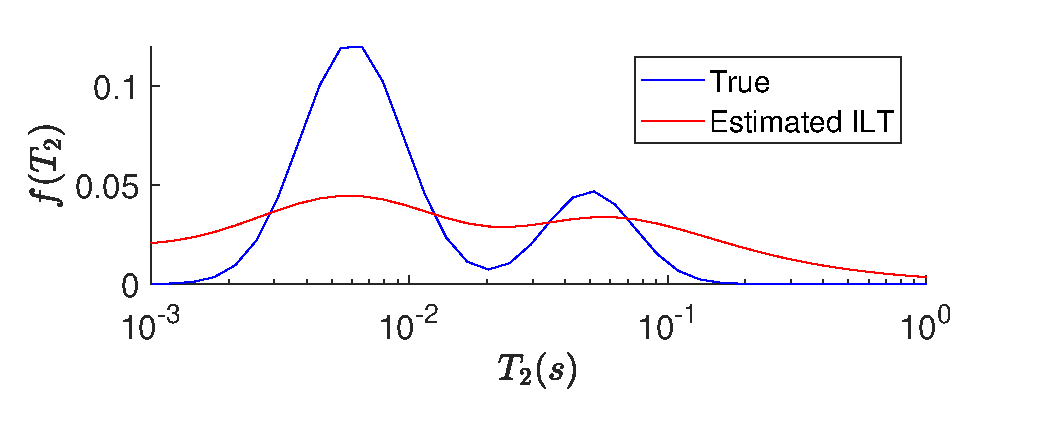
\includegraphics[width=0.6\textwidth]{backgroundVector/iltOptimise.eps}
    \caption{Application of the ILT inversion of measured data on the model.}
    \label{fig:2002ILTSimulation}
\end{figure}


\subsection{The Moment Estimator}
Evaluating the performance of the moment estimation involves comparing between the moments of the original density function, 
\begin{enumerate}
    \item the moments estimated with the Mellin transform, and
    \item the moments computed from the estimated distribution using the ILT.
\end{enumerate}
The accuracy of the moment estimator is measured using the normalised root mean square error ($NRMSE$) \cite{GruberT2Estimation2013} between the mean of the estimate and the true value.
\begin{equation}
    NRMSE = 100 \times
    \frac
    {\sqrt{(\mu_{\text{est}} - \mu_{\text{true}})^2}}
    {\mu_{\text{true}}}
    \label{eq:defnNRMSE}
\end{equation}

\begin{figure}[t]
    \centering
    \begin{subfigure}[b]{0.49\textwidth}
        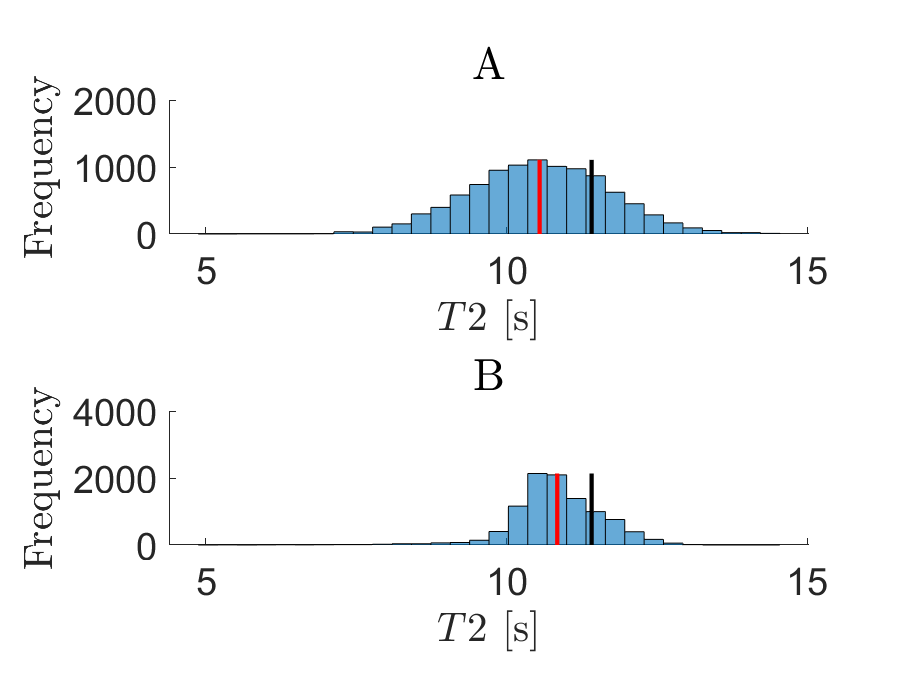
\includegraphics[width=\textwidth]{backgroundVector/moment-5e-1.eps}
        \subcaption{Estimation of the $-0.5^{th}$ moment of $f(T_2)$}
        \label{fig:moment5e-1Estimate}
    \end{subfigure}
    \begin{subfigure}[b]{0.49\textwidth}
        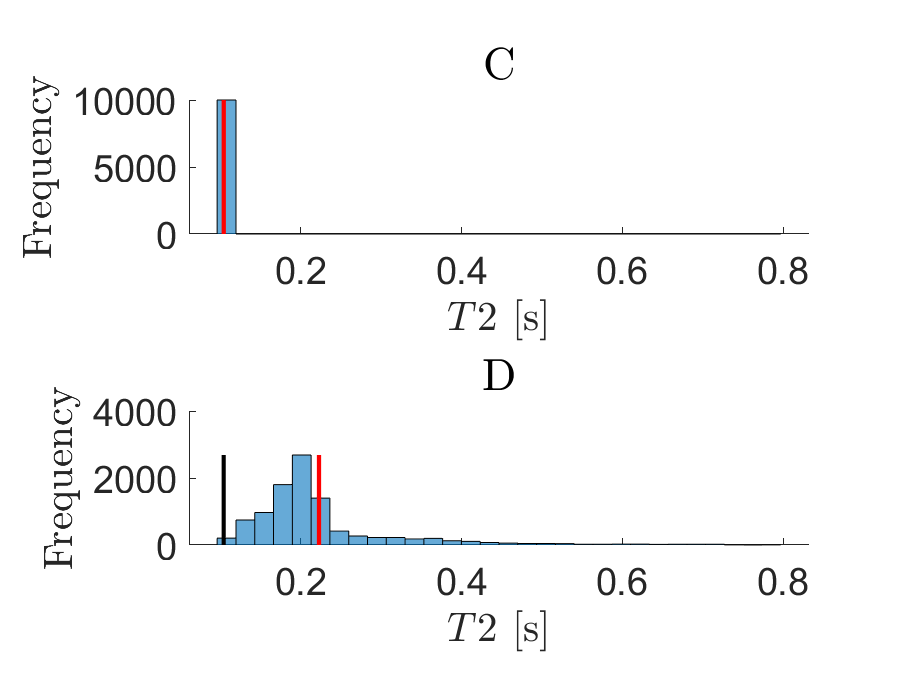
\includegraphics[width=\textwidth]{backgroundVector/moment5e-1.eps}
        \subcaption{Estimation of the $0.5^{th}$ moment of $f(T_2)$}
        \label{fig:moment1Estimate}
    \end{subfigure}
    
    \caption{The performance of the MT (A, C) compared to the ILT (B, D) in estimating the moments of the density function. Red is the mean of the estimated moment and black is the true moment.}
    \label{fig:estimateMoments}
\end{figure}
Figure \ref{fig:estimateMoments} demonstrates the performance of the Mellin transform versus the ILT for 10,000 different simulations. We see that the MT has a higher $NRMSE$ than the ILT for negative values of $\omega$. For higher values we see that the $NRMSE$ is significantly lower for the MT compared to the classic ILT.

\subsection {The Tapered Area Estimator}

Using the same methodology as moment estimation, the $NRMSE$ is used to quantify the accuracy of the EHT compared to the ILT (Fig. \ref{fig:estimateTaperedAreas}). We see that the EHT tapered area estimations have a significantly lower spread compared to the ILT. Furthermore, the $NRMSE$ of the EHT is typically smaller than the $NRMSE$ of the ILT method.

\begin{figure}
    \centering
    \begin{subfigure}[b]{0.49\textwidth}
        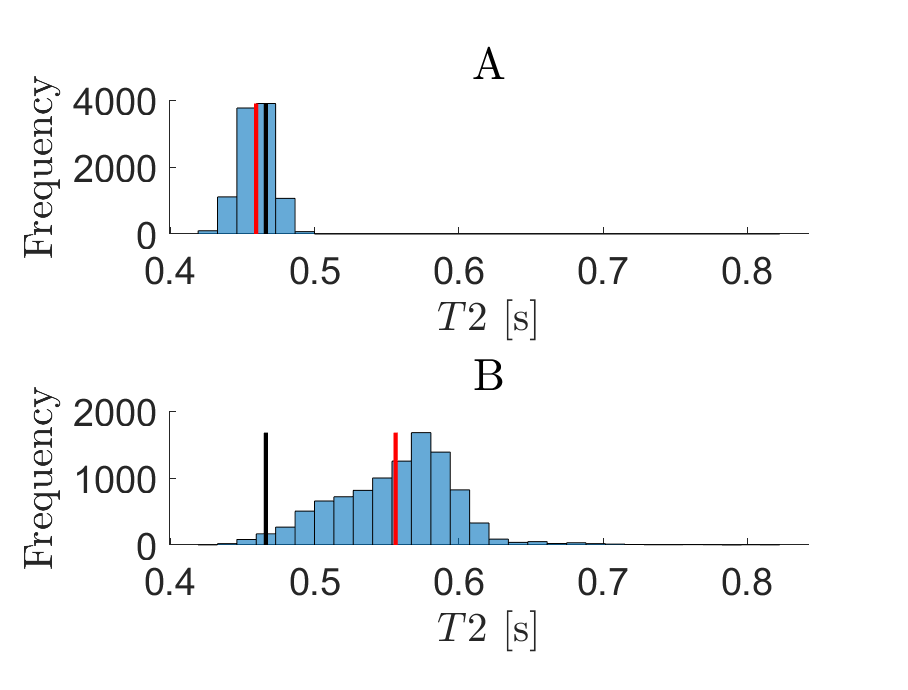
\includegraphics[width=\textwidth]{backgroundVector/area1e-2.eps}
        \subcaption{Estimation of the tapered area where $T_c = 0.01$ seconds}
        \label{fig:estTaperedAreaTc1e-1}
    \end{subfigure}
    \begin{subfigure}[b]{0.49\textwidth}
        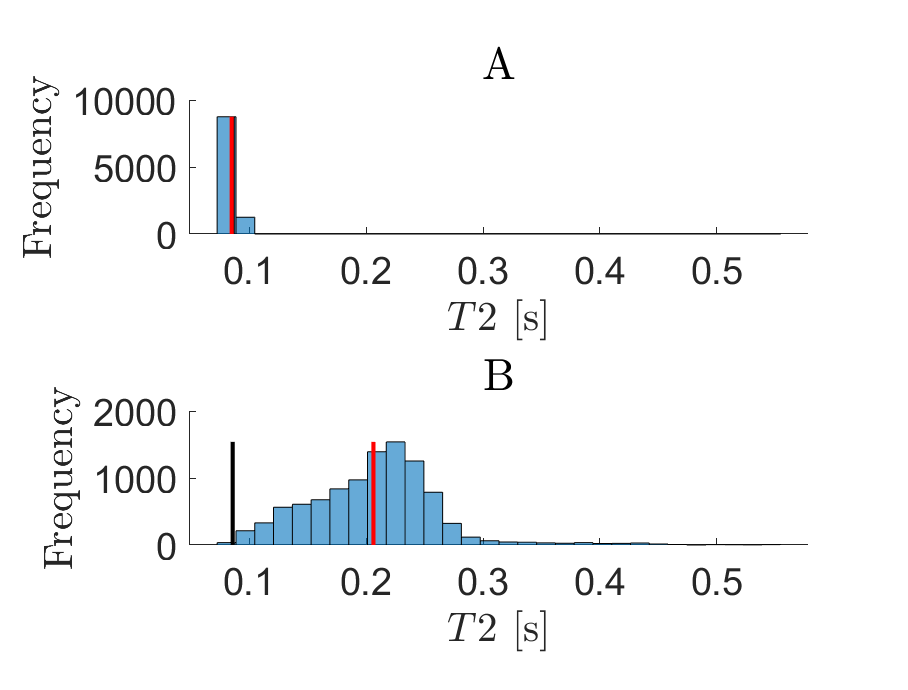
\includegraphics[width=\textwidth]{backgroundVector/area1e-1.eps}
        \subcaption{Estimation of the tapered area where $T_c = 0.1$ seconds}
        \label{fig:estTaperedAreaTc1}
    \end{subfigure}
    \caption{The performance of the EHT (A, C) compared to the ILT (B, D) in estimating the tapered area of the density function. Red is the mean of the estimated area and black is the true area.}
    \label{fig:estimateTaperedAreas}
\end{figure}


\subsection {The ILT+ Method}

The two metrics that were used to evaluate and compare this method with the ILT are:
\begin{itemize}
    \item the $NRMSE$ of the logarithmic mean ($T_{2_{LM}}$), and
    \item the $NRMSE$ of the bound fluid volume ($BFV$), with $T_c = 0.033 $s for sandstone \cite{TaperedAreaskleinberg1997tapered} \cite{wellLoggingBook}.
\end{itemize}

\paragraph{}
The use of linear functionals in the optimisation framework leads to more precise and accurate estimations of density function's properties \cite{GruberT2Estimation2013}. We see in figure \ref{fig:logMeanILT+} that the ILT+ method provides decreased bias and variance in predicting the logarithmic mean compared to the classic ILT. The error ($NRMSE$) is reduced with the introduction of linear functionals. Figure \ref{fig:BFVILT+} demonstrates that the ILT+ method also provides more accuracy and precision for predicting the bound fluid volume of a sample.

\begin{figure}[ht!]
    \centering
    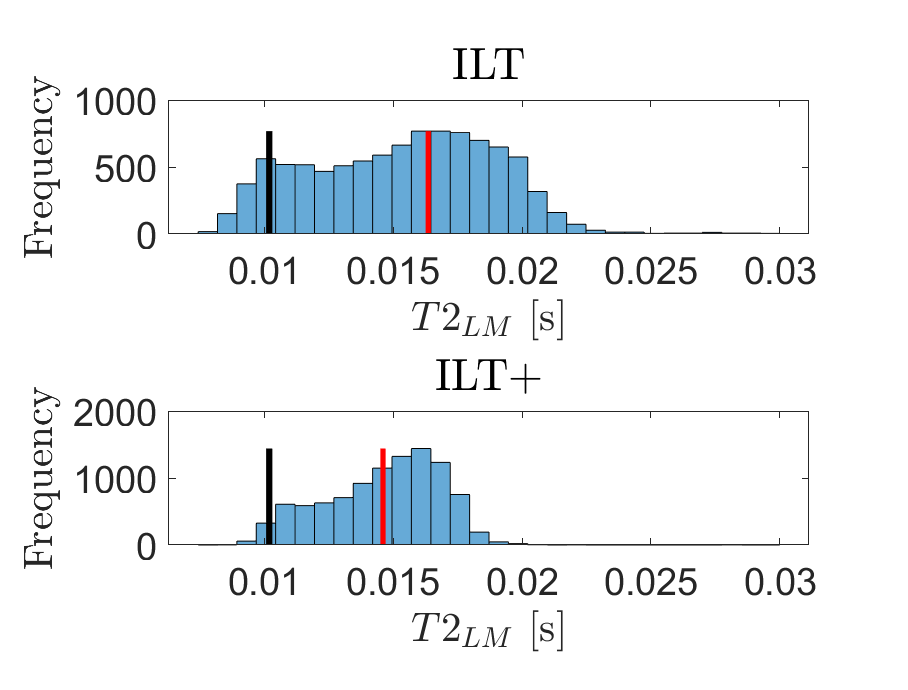
\includegraphics[width=0.5\textwidth]{backgroundVector/logMeanSimulate.eps}
    \caption{Estimation of the logarithmic mean directly from estimated distributions. Estimations by ILT and ILT+ are shown in plots A and B respectively. The black line is the true value and the red line is the estimated value.}
    \label{fig:logMeanILT+}
\end{figure}

\begin{figure}[ht!]
    \centering
    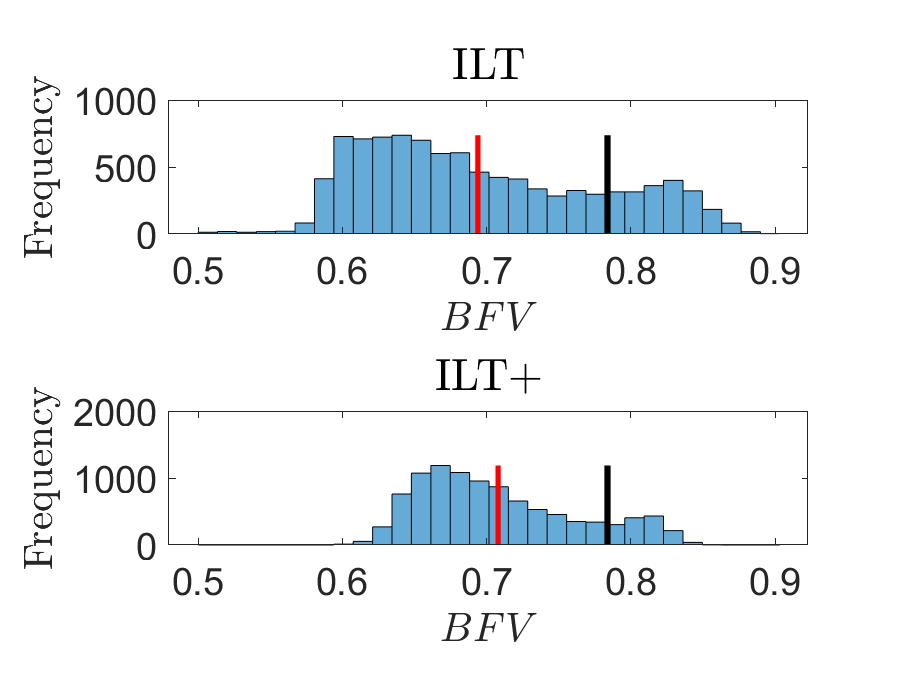
\includegraphics[width=0.5\textwidth]{backgroundVector/bfvSimulate.eps}
    \caption{Estimation of the bound fluid volume directly from estimated distributions. Estimations by ILT and ILT+ are shown in plots A and B respectively. The black line is the true value and the red line is the estimated value.}
    \label{fig:BFVILT+}
\end{figure}

These results make the ILT+ technique the benchmark to beat for this project`s proposed Bayesian method.
    
    
    










